%% LyX 2.3.1 created this file.  For more info, see http://www.lyx.org/.
%% Do not edit unless you really know what you are doing.
\documentclass[12pt,english]{kuthesis}
\usepackage{mathptmx}
\usepackage[T1]{fontenc}
\usepackage[utf8]{inputenc}
\usepackage{geometry}
\geometry{verbose,tmargin=1in,bmargin=1in,lmargin=1in,rmargin=1in}
\setcounter{secnumdepth}{3}
\setcounter{tocdepth}{3}
\setlength{\parskip}{\smallskipamount}
\setlength{\parindent}{0pt}
\usepackage{graphicx}
\usepackage[authoryear]{natbib}

\makeatletter

%%%%%%%%%%%%%%%%%%%%%%%%%%%%%% LyX specific LaTeX commands.
%% Because html converters don't know tabularnewline
\providecommand{\tabularnewline}{\\}

%%%%%%%%%%%%%%%%%%%%%%%%%%%%%% User specified LaTeX commands.
%%\usepackage{latexsym}
\usepackage{graphicx}

%%\usepackage{psfig}
%%\usepackage{color}

%%%%%%%%%%%%%%%%%%%%%%%%%%%%%% User specified LaTeX commands.
\usepackage{ragged2e}
\RaggedRight
%\setlength{\parindent}{1.5 em}

\makeatother

\usepackage{babel}
\begin{document}

\chapter{Ordinal Outcomes Regression}

\begin{chapterabstract}
On January 19, 2019, the environment "chapterabstract" was introduced.  This was a frequent request from science-department users, whose advisors wanted the chapters to be more-or-less directly imported from published article markup. 
\end{chapterabstract}

\section{Introduction}

This is my best effort to succinctly explain the theory behind the
ordinal logistic regression model (with apologies to the probit model). 

The main takeaway point is supposed to be this: 
\begin{quote}
The same data leads to different estimates from different programs.
That happens because the ordinal model can be written down in several
different ways. None of them are wrong, but they are different, and
as a result the user must be cautious.
\end{quote}
Estimates obtained from four different programs are offered in Table
\ref{tab:Ordinal-Regression-Results}. If we line these up side by
side, we see that estimates from one of the routines for R matches
Stata (after chopping off the small differences in the decimals),
while SAS appears to provide the ``wrong sign'' for the first row
and the second procedure for R seems to provide the ``wrong signs''
for the second and third rows.

\begin{table}

\caption{Ordinal Regression Results\label{tab:Ordinal-Regression-Results}}

\centering{}%
\begin{tabular}{|c|c|c|c|c|}
\hline 
 & R: polr & R: lrm & SAS & Stata\tabularnewline
\hline 
\hline 
$\hat{b}_{1}$ & -0.28 & -0.28 & 0.28 & -0.28\tabularnewline
\hline 
$\hat{\zeta}_{1}$ & -4.24 & 4.24 & -4.24 & -4.24\tabularnewline
\hline 
$\hat{\zeta}_{2}$ & -2.32 & 2.32 & -2.32 & -2.32\tabularnewline
\hline 
\end{tabular}
\end{table}
None of these are actually wrong, they are all correct \emph{given
the model they specified}. This the point at which the student may
be tempted to give up. Please don't. I've worked very hard to clear
this up in the following sections.

\section{Extending the Logit Model to deal with Ordinal Dependent Variables}

The easiest way to understand regression with ordinal dependent variables
is to extend the ``cumulative probability interpretation'' of the
two category model \citep{pinheiro_mixed-effects_2000}. 

In the two category model, $y_{i}$ is 1 with probability 
\begin{equation}
F(b_{0}+b_{1}X_{i})=\int_{-\infty}^{b_{0}+b_{1}X_{i}}f(e_{i})de_{i}
\end{equation}
And, of course, the probability that $y_{i}$ is 0 will be $1-F(b_{0}+b_{1}X_{i}).$
The formula $F$ is a ``cumulative distribution function'' (CDF),
it represents the probability that a random variable $e_{i}$ will
be as small or smaller than $b_{0}+b_{1}X_{i}$. The function $f$
is a ``probability density function'' (PDF), which represents the
probability that $e_{i}$ is equal to some particular value. This
is illustrated in Figure \ref{fig:Dichotomous}. The ``probability
density function'' $f$ is defined from left to right and the possible
outcomes are divided into two sets by the line drawn at $e_{i}=b_{0}+b_{1}X_{i}$.
The area under the curve on the left side is the probability of getting
a ``yes'' (or 1). The area on the right is the chance of a ``no''
(0).

\begin{figure}
\begin{centering}
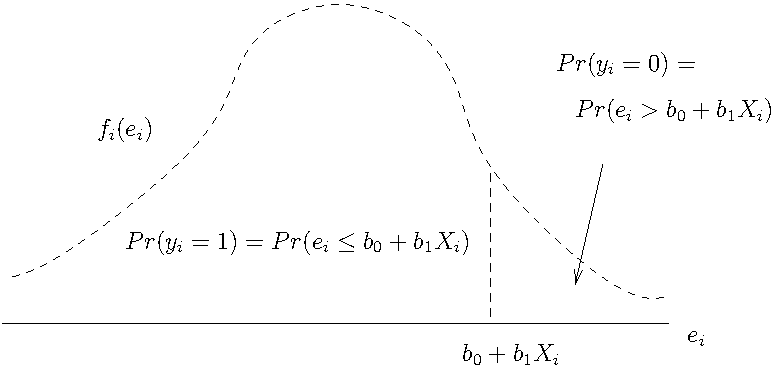
\includegraphics{ordinal-fig-1}
\par\end{centering}
\caption{Dichotomous Outcome Variable\label{fig:Dichotomous}}
\end{figure}
Suppose $y_{i}$ can have $3$ values, $0$, $1$, and $2$. (Keep
in mind that this model can be written down in several ways. We tackle
my favorite first, and then consider the others.) Leave the predictive
part of the model ($b_{0}+b_{1}X_{i})$ the same, but we now introduce
two new positive constants ($\Pi_{0}$ and $\Pi_{1}$) that divide
the space. Considering Figure \ref{cap:Ordinal-Logit}, it should
be easy to see why some people call these new parameters ``thresholds''. 

\begin{figure}
\begin{centering}
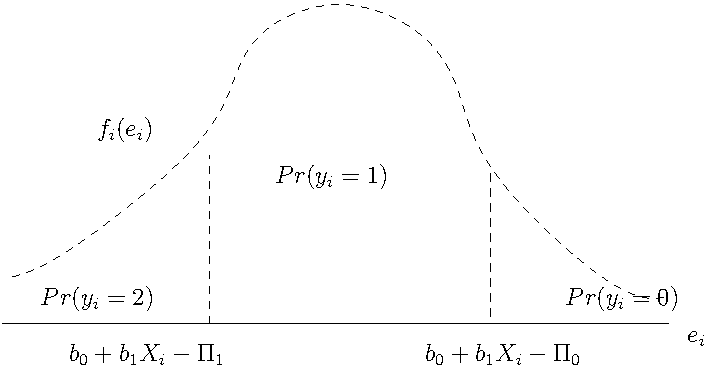
\includegraphics{cumulative2}
\par\end{centering}
\caption{Ordinal Logit\label{cap:Ordinal-Logit}}
\end{figure}
To summarize the effect of these new thresholds, we write down 1 equation
for each possible outcome. My tendency is to write the thresholds
as positive values like so:

\begin{equation}
y_{i}=\left\{ \begin{array}{lll}
2 & if\,b_{0}+b_{1}X_{i}-e_{i}\geq\Pi_{1}\\
1 & if\,\Pi_{0}\leq b_{0}+b_{1}X_{i}-e_{i}<\Pi_{1}\\
0 & if\,b_{0}+b_{1}X_{i}-e_{i}<\Pi_{0}
\end{array}\right.\label{eq:3category1}
\end{equation}

Note we don't really need 3 equations. If we have two, say $Pr(y_{i}=0)$
and $Pr(y_{i}=1)$, then the chance of ending up in the other category
is $1-Pr(y_{i}=0)-Pr(y_{i}=1)$.

In order to translate this into a model involving the cumulative probability
distribution, re-arrange so that the random variable $e_{i}$ is by
itself.

\begin{equation}
y_{i}=\left\{ \begin{array}{lll}
2 & if\,e_{i}\leq b_{0}+b_{1}X_{i}-\Pi_{1}\\
1 & if\,b_{0}+b_{1}X_{i}-\Pi_{1}<e_{i}\leq b_{0}+b_{1}X_{i}-\Pi_{0}\\
0 & if\,b_{0}+b_{1}X_{i}-\Pi_{0}<e_{i}
\end{array}\right.\label{eq:3category2-1}
\end{equation}

As in the dichotomous case, the probabilities of the various outcomes
are calculated by use of cumulative probability. Rearrange \ref{eq:3category1}
to convert these into probabilities of the individual outcomes.

\begin{equation}
\begin{array}{lll}
Pr(y_{i}=2) & =Pr(e_{i}\leq b_{0}+b_{1}X_{i}-\Pi_{1}) & =F(b_{0}+b_{1}X_{i}-\Pi_{1})\\
Pr(y_{i}=1) & =Pr(b_{0}+b_{1}X_{i}-\Pi_{1}\leq e_{i}<b_{0}+b_{1}X_{i}-\Pi_{0})\\
 & =1-F(b_{0}+b_{1}X_{i}-\Pi_{0})-F(b_{0}+b_{1}X_{i}-\Pi_{1})\\
Pr(y_{i}=0) & =Pr(b_{0}+b_{1}X_{i}-\Pi_{0}<e_{i}) & =1-F(b_{0}+b_{1}X_{i}-\Pi_{0})
\end{array}\label{eq:3category2}
\end{equation}
\\
Note that any one category can be thought of as a ``residual'' category
after the others have been assigned their shares. The middle category,
$y_{i}=1,$ is left over if we ``chop off'' the outcomes on the
left ($y_{i}=2$) and the right ($y_{i}=0$). We are left with the
chance of ending up in the middle. In that sense, the probability
of landing in the middle is equal to $1.0$ minus the chance of a
very small amount of random noise ($e_{i}\leq b_{0}+b_{1}X_{i}-\Pi_{1}$)
and minus the chance of having a very large random noise ($b_{0}+b_{1}X_{i}-\Pi_{0}<e_{i}$).
Similarly, the chances of being in the top category equal $1$ minus
the chance of ending up in the lower categories.

Any probability distribution can be used for the random error $e_{i}$,
the two most common being Logistic and Normal. If the Normal is chosen,
it is customary to call this a ``probit'' model and the symbol for
the cumulative distribution is usually $\Phi()$.

What if your dependent variable have more categories? Add more thresholds!
See the example in Figure \ref{fig:Ordinal-5cat}.

\begin{figure}
\begin{centering}
\par\end{centering}
\begin{centering}
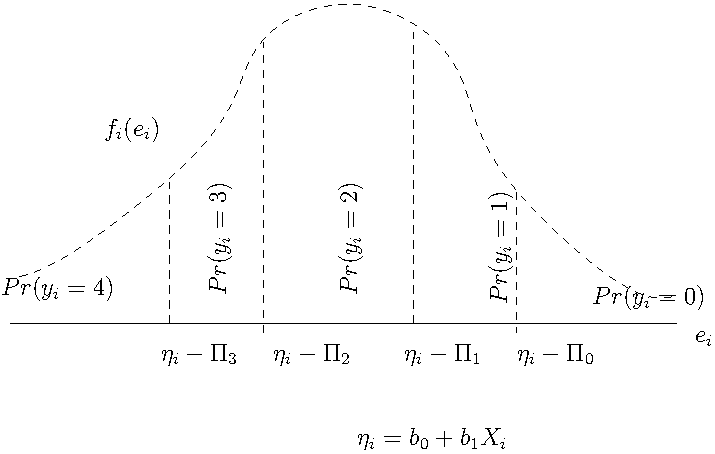
\includegraphics{ordinal-fig-3}
\par\end{centering}
\caption{Ordinal Model with More Categories\label{fig:Ordinal-5cat}}
\end{figure}

\end{document}
